\documentclass[paper=A4,
  pagesize=auto,
  fontsize=12pt,
  numbers=noenddot, 
  bibliography=totoc,
  abstract=off,
  DIV=calc,
  headsepline,
  headinclude=true,
  footinclude=false,
  cleardoublepage=plain,
  captions=tableheading,
  draft=false,
  open=right,
  BCOR=1cm,
  toc=graduated,
  english
]{scrreprt}
\usepackage{graphicx, color}
\usepackage{fixltx2e}

% ========= Sprache, Font und Kodierung =========
  \pdfprotrudechars=2
  \pdfadjustspacing=2

  \usepackage{amsmath}
\usepackage{mathptmx} % kompakte Schriftfont
  \usepackage[english]{babel}
  \usepackage[utf8]{inputenc}
  %\usepackage[ngerman=ngerman-x-latest]{hyphsubst}
  \usepackage{csquotes} 

  \usepackage{ragged2e}
  \usepackage{setspace}
% ========= Sprache, Font und Kodierung =========



% ========= LaTeX, Formatierung, Layout =========
  %\usepackage{amssymb} % Einige Sonderzeichen
  \usepackage{ifthen} % Paket für if-then-else-Konstrukte
  \usepackage{array}     % weitere Hilfsmittel für Tabellen
  \usepackage{booktabs}
  \usepackage{threeparttable}
  \usepackage{etoolbox}
  \appto\TPTnoteSettings{\footnotesize}
  \usepackage{scrhack} % Beinhaltet einen notwendigen Fix
  \usepackage[shortcuts]{extdash}
  \usepackage{xspace}
  \usepackage[text={13cm,20cm}]{geometry} % Seitenlayout /Textboxgröße
% ========= LaTeX, Formatierung, Layout =========


% ============== Literaturverzeichnis ==============
\usepackage[%
  backend=biber,
  style=authoryear-icomp,
  bibstyle=numeric,
  citestyle=numeric-comp,
  maxnames=3,
  url=false,
  eprint=false,
  doi=false,
  isbn=false,
  sorting=none
]{biblatex}
\bibliography{refs}

% ============== Literaturverzeichnis ==============

% ==================== Floats ====================
  \usepackage{float}
  \usepackage[section]{placeins}
  \usepackage{flafter}
  \usepackage{caption}[2012/02/19]
  \usepackage{subcaption}
  %\usepackage[font=small]{subcaption}
  \floatstyle{ruled}
  \captionsetup{
    format=plain,
    margin=10pt,
    font=small,
    labelfont=bf,
    labelsep=endash
  }

% ==================== Floats ====================

% ================= Definitionen =================
  \usepackage{amssymb}
  \usepackage{xspace}
  %\usepackage{siunitx} % Paket für physikalische Einheiten
  \usepackage{appendix}
  \renewcommand{\appendixtocname}{Anhang}
  \usepackage{paralist} % Mehr Listenumgebungen
  \usepackage{textcomp}
  \usepackage{multirow}
% ================= Definitionen =================

% =================== Hyperref ===================
    %\definecolor{myLinkColor}{rgb}{0,0,0}
    %\definecolor{myCiteColor}{rgb}{0,0,0}
    %\definecolor{myFileColor}{rgb}{0,0,0}
    %\definecolor{myURLColor}{rgb}{0,0,0}
  \usepackage[hidelinks,breaklinks]{hyperref}
  %\setcounter{biburllcpenalty}{100}
  %  \pdfcompresslevel=9 %Kompressionslevel fuer Text und Grafiken
  %  \DeclareGraphicsExtensions{.pdf, .png, .jpg, .tif, .mps} % Dateiendungen für Grafikdateien, geordnet nach Priorität für automatische Auswahl der richtigen Datei, falls Endung nicht angegeben 
% =================== Hyperref ===================

% =================== Glossar ====================
  \usepackage[acronym,nonumberlist,nopostdot,nomain,style=long]{glossaries}
  %\usepackage[acronym,nonumberlist,nopostdot,style=long]{glossaries}
  \setlength{\glsdescwidth}{0.8\linewidth}
  \loadglsentries[acronym]{abbreviations}
  \glsaddall
  \makeglossaries
  %\usepackage{makeidx}
  %\makeindex
% =================== Glossar ====================

\usepackage{ellipsis} % Muss nach Hyperref
\usepackage{todonotes}
%%---Silbentrennung-----------------------------------------------------------------------------

% Silbentrennung für Wörter, in denen kein Bindestrich vorkommt
\hyphenation{
Bei-spiel
} 
%----------------------------------------------------------------------------------------------


\sloppy


% =================== Unterschrift ===============
\newcommand{\doubleSignature}[2]{
\begin{minipage}[c]{\textwidth}
\vspace{2cm}

\makebox[12cm][c]{
 #1, xx.xx.2016 
}
\vspace{3cm}

\makebox[12cm][c]{
 \hrule{12cm}{0mm}
}
\makebox[12cm][c]{
 #2
}
\vspace{1cm}
\end{minipage}
}
\newcommand*{\SignatureAndDate}[1]{%
    \par\noindent\makebox[2.5in]{\hrulefill} \hfill\makebox[2.0in]{\hrulefill}%
    \par\noindent\makebox[2.5in][l]{#1}      \hfill\makebox[2.0in][l]{Date}%
}%


\begin{document}

\pagenumbering{gobble}

\begin{titlepage}
    \centering
    \vspace*{3cm}

    Genome Informatics, Faculty of Technology\\[10pt]
    {\Large\textbf{PragIG: Probabilistic Reconstruction of Ancestral Gene order using Intermediate Genomes}\\[40pt]}
      
    Master Thesis\\[6pt]
    for attainment of the academic degree of\\[6pt]
    {\Large\textbf{Master of Science}}\\[6pt]
    presented by\\
    Kevin Lamkiewicz\\
    {\small Bioinformatics and Genome Research\\
    Faculty of Technology, Bielefeld University}\\[40pt]
    
    \textbf{Supervisors}\\[10pt]
    Dr.~Pedro Feijão \\
    \rule{15em}{0.4pt}\\[1\baselineskip]
    Prof.~Dr.~Jens Stoye \\
    \rule{15em}{0.4pt}\\[1\baselineskip]
    \vspace{1\baselineskip}
    \vfill
    Bielefeld University\\
    Universitätsstraße 25, 33615 Bielefeld\\
    \vfill
    01.09.2016\par
    \vfill 
\end{titlepage}

\newpage
 \begin{centering}
 \chapter*{Statement of Authentication}
 \end{centering} \noindent
  I hereby declare that I have written the present thesis independently, without assistance
  from external parties and without use of other resources than those indicated. The ideas
  taken directly or indirectly from external sources (including electronic sources) are duly
  acknowledged in the text. The material, either in full or in part, has not been previously
  submitted for grading at this academic institution. \\ \bigskip\bigskip\bigskip
 \SignatureAndDate{Kevin Lamkiewicz}
\newpage

\tableofcontents

\cleardoubleemptypage

\pagenumbering{arabic}
\setcounter{page}{3}
\chapter{Summary}
Evolutionary biologists are trying to reconstruct genomes of extinct ancestral species.
All genetic information is subject to continuous changes called mutations.
Mutations are not only made up at the level of base-pair changes but also by rearrangement events such as inversions,
translocations, fusions and fissions~\cite{Kent30092003}.
\\ \ \\
In order to model these events, a notation from previous work is used~\cite{Bergeron2006}.
Let $g$ be a conserved region (\emph{gene}) in a genome.
Each gene has two extremities, the tail ($g^t$) and the head ($g^h$).
We write $g$ ($-g$) if along the chromosome the tail of $g$ comes before (after) its head.
Two adjacent extremities of two consecutive genes form an \emph{adjacency}.
Considering linear chromosomes, an extremity without an adjacent extremity is called \emph{telomere}.
One rearrangement model that considers the most common rearrangement events is the \emph{\gls{dcj}} model~\cite{Yancopoulos15082005}.
\\ \ \\
In order to reconstruct ancestral gene orders, internal nodes of a given phylogenetic tree, with extant genomes at the leaves, have to be labeled
with the ancestral genomes in a way such that the cost of the resulting tree is minimized.
This is also known as the \emph{\gls{spp}}. 
Over the past few years, different methods to reconstruct ancestral gene orders have been proposed.
These methods can be divided into two groups: event-based methods and homology-based methods.
Event-based methods use rearrangement models and scenarios to reconstruct the ancestral genome.\\
Transforming one genome into another with the help of rearrangements is also called \emph{sorting}.
Every series of rearrangement operations that transforms genome $A$ into $B$ is a \emph{valid sorting scenario}.
However, it has been shown that the solution space of sorting with \gls{dcj} grows exponentially with the distance of the genomes to be sorted~\cite{Stoye2010}.
Furthermore, solving the \gls{spp} under the \gls{dcj} model is NP-hard~\cite{Tannier2009}.
\\ \ \\
Recently Feijão~\cite{Feijao2015} proposed a new heuristic that solves the \gls{spp} under \gls{dcj}.
For that, he used the \emph{\gls{cbp}} that visualizes the rearrangement events between two genomes $A$ and $B$.
Using the \gls{dcj} model in order to calculate optimal sorting scenarios exploits the advantage of the \gls{cbp}
where every component of the graph is a cycle.
The goal in that work is to find intermediate genomes of two genomes $A$ and $B$ that arise in optimal sorting scenarios.
Labeling the internal nodes of the phylogenetic tree with intermediate genomes improves the ancestral reconstruction results, even though the tree itself
might not be the most parsimonious one~\cite{Feijao2015}.
\\ \ \\
\todo{Dieser Abschnitt muss zum Schluss neu geschrieben werden!}\\
\todo{Kurzen Absatz über die Aufteilung der Masterarbeit}
In the scope of my master thesis I want to extend the method of Feijão by a probabilistic approach.
This approach considers the probability of an adjacency being affected by a rearrangement.
Similar approaches have been proposed for event-based methods already~\cite{Ma2006,Yang2014,Hu2013}, however the framework of Feijão is able to 
add information about homology. 
With this information, we think we are able to improve the probabilistic approaches.\\
Another point I would like to study is the positional constraint of genes.
Swenson and Blanchette~\cite{Swenson2015} showed how to color adjacency graphs considering the position of genes \emph{in vivo}.
These positional constraints could improve the probability approach even further.
\chapter{Introduction}



\section{Modeling genomes} % (fold)
\label{sub:modeling_genomes}

Multichromosomal genomes are represented using a notation as in previous work~\cite{Bergeron2006}.\\
A chromosome is represented by a sequences of genes.
If the chromosome is \emph{linear} it is flanked by \emph{telomeres} ($\circ$).
A genome $G$ is the set of its chromosome.
A gene $g$ from $G$ has two extremeties, the tail ($g^t$) and the head ($g^h$).
Since genes can be located both DNA strands, we encode this by a leading $-$, i.e. $g$ is located on the leading strand and $-h$ on the lagging strand.
It is possible to describe \emph{adjacencies} between two genes $g$ and $h$. 
If $g$ and $h$ are two consecutive genes in the genome $G$, we can describe their adjacency by their adjacent gene extremeties.
Note that there exist four different ways of orientation for two genes.
Gene extremeties that are located on the end of a linear chromosome are often combined with the telomere, thus forming a \todo{Rausstreichen} \emph{telomeric adjacency}. 
In order to describe a genome $G$ it is possible to use the set of chromosomes or the set of adjacencies $A$.\\
The genome $G_A$ in Figure~\ref{fig:genomeRep} has two linear chromosomes with five genes, where $G_A=\{(\circ\ 1\ -2\ 3\ \circ),(\circ\ 4\ 5\ \circ)\}$
and $A=\{\circ 1^t, 1^h2^h, 2^t3^t, 3^h\circ, \circ 4^t, 4^h5^t, 5^h\circ\}$\\ \ \\

\begin{figure}[h]
	\centering
	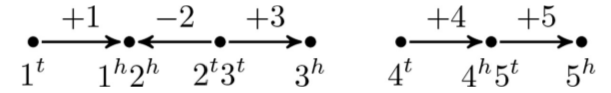
\includegraphics[scale=0.4]{figures/genomeRep.png}
	\caption{%
	 The Genome $G_A=\{(\circ\ 1\ -2\ 3\ \circ),(\circ\ 4\ 5\ \circ)\}$ with its corresponding adjacency set 
	 $A=\{\circ 1^t, 1^h2^h, 2^t3^t, 3^h\circ, \circ 4^t, 4^h5^t, 5^h\circ\}$.  
	 Figure taken from~\cite{Feijao2015}
		}%
	\label{fig:genomeRep}
\end{figure}
\noindent
Given two genomes $A$ and $B$ with the same set of genes, the \emph{breakpoint graph} $BP(A,B)$ is defined in the following way~\cite{Tannier2009}:\\
Let $G=BP(A,B)$ be a graph where the vertex set $V(G)$ is the set of gene extremities and the edge set $E(G)$ the set of non-telomeric
adjacencies of $A$ and $B$.
The edges are also called \emph{A-edges} and \emph{B-edges} respectively. \\ \ \\
It is common to draw the adjacencies from $A$ and $B$ in different colors within the breakpoint graph.
Each component in $BP(A,B)$ is either a cycle, an even path or an odd path.
The parity of a path is defined by the \emph{size} of a component, where the size is the number of vertices in the component.\\
An example for a breakpoint graph $BP(A,B)$ with two genomes $A$ and $B$ is given in Figure~\ref{fig:BPgraph}.

\begin{figure}[h]
	\centering
	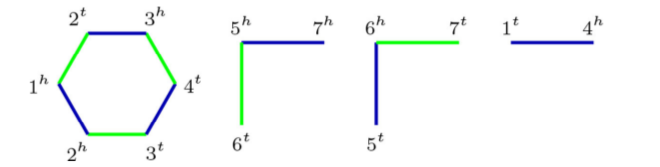
\includegraphics[scale=0.5]{figures/BPG_1.png}
	\caption{%
		Breakpoint Graph $BP(A,B)$ of $A=\{\circ 1^t,1^h2^t,2^h3^t,3^h4^t,4^h\circ,\\\circ 5^t,5^h6^t,6^h7^t,7^h\circ\}$ and 
		$B=\{1^h2^h,2^t3^h,3^t4^t,4^h1^t,\circ 6^t,6^h5^t,5^h7^h,7^t\circ\}$.
		A-edges are green, B-edges are blue. Figure taken from~\cite{Feijao2015}.
	}%
	\label{fig:BPgraph}
\end{figure}

% section modeling_genomes (end)

\section{DCJ model} % (fold)
\label{sub:dcj_model}
The \emph{Double-Cut-and-Join} (DCJ) operation rearranges the order of genes by cutting two adjacencies and rejoining the affected extremities
in another way.
It is shown that the DCJ distance $d(A,B)$ for two genomes $A$ and $B$ can be determined using the Breakpoint Graph $BP(A,B)$~\cite{Bergeron2006}:
\[
	d(A,B) = n - c - \frac{o}{2}
\]
where $n$ is the number of genes, $c$ and $o$ are the number of cycles and odd paths in the Breakpoint Graph, respectively.\\
It is also shown that each \emph{component} can be considered independently in order to calculate the DCJ distance~\cite{Stoye2010}.\\

% section dcj_model (end)

\section{Circular Breakpoint Graph} % (fold)
\label{sub:circular_breakpoint_graph}
In order to simplify the calculation of the \emph{DCJ-distance} the Breakpoint Graph is extended to a \emph{Circular Breakpoint Graph}~\cite{Feijao2015}.
For each odd and even path in $BP(A,B)$ telomeres are added and connected in a way, such that each \emph{telomeric adjacency} in the Breakpoint Graph
is connected to a telomere. Please reconsider the example of a Breakpoint Graph in Figure~\ref{fig:BPgraph}.
The extended version to the Circular Breakpoint Graph is shown in Figure~\ref{fig:cBPgraph}.

\begin{figure}[h]
	\centering
	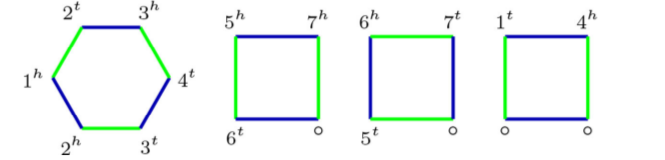
\includegraphics[scale=0.5]{figures/cBPG.png}
	\caption{%
	 Circular BP graph of the BP(A,B) from Figure~\ref{fig:BPgraph}. \emph{A-edges} are drawn in green, \emph{B-edges} are drawn in blue.
	 Figure taken from~\cite{Feijao2015}.
	}%
	\label{fig:cBPgraph}
\end{figure}

During the rest of this thesis the term Breakpoint Graph or $BP(A,B)$ refers to the circular version.

\pagenumbering{roman}
\chapter*{Acknowledgment}
Has to be done in the end.
%\newpage
\printglossaries

\newpage
\printbibliography

\end{document}